\documentclass[sigconf]{acmart}
\settopmatter{printacmref=false}

\renewcommand\footnotetextcopyrightpermission[1]{}

\pagestyle{plain}

\usepackage{booktabs} % For formal tables
\usepackage{hyperref}
\usepackage[]{algorithm2e}
\usepackage{graphicx} % support the \includegraphics command and options
\graphicspath{{./images/}}


\begin{document}
\title{Computational Intelligence Coursework}
\acmConference[SET10107]{Coursework}{April 2022}{Edinburgh Napier University} 
\acmYear{2022}
\copyrightyear{2022}

\author{40451571 Connor Timmins}



\begin{abstract}This coursework requires the weights of a multi-layer perceptron artifical neural network to be evolved and used to control the landing of spacecraft. To achieve this, an evolutionary algorithm was implemented. Multiple operators were applied and tested to find the best methods for this problem. Parameter tuning was performed to further satisfy our goals of finding the best combination for safe landing.
\end{abstract}



%\keywords{ACM proceedings, \LaTeX, text tagging}


\maketitle

\section{Approach}
\subsection{Algorithm}
To solve this problem, we employed a steady state evolutionary algorithm \cite{SteadyState}.
The steady state evolutionary algorithm uses the following structure: Individuals are initialised and a loop of selection, crossover, mutation and replacement operations occur until a stopping criteria is met. In this paper, we document experiments on the selection, crossover, mutation and replacement operations with the intent of finding the combination of operators that lead to the best fitness value.

We choose to use a Steady State algorithm as its simplicity allow us to focus on experimenting with operators and parameters. We run all experiments for 20000 generations to allow these operators ample time to display their effects and the faster runtime provided by Steady State over a simple evolutionary algorithm which replaces more of their population each generation allows us to better understand that effect without causing prohibitively long runtimes.

\begin{algorithm}
INITIALISE population with randomly generated individuals\;
EVALUATE every individual\;
 \While{Termination Condition is not satisfied}{
SELECT parents\;
RECOMBINATION to produce offspring\;
MUTATE the offspring\;
EVALUATE the offspring\;
REPLACE worst individuals in population with offspring\;
}
\caption{Steady State Algorithm}
\end{algorithm}

\subsection{Operators}
\subsubsection{Selection}
The first operation taken in the reproductive cycle of the algorithm is selection. This operation selects parent individuals from the population which will be subsequently used to create new child individuals. A good selection operator will select parents which cause the population to trend towards a high fitness without causing a premature convergence. The following selection operators were implemented and tested:
\begin{description}
\item[Fitness Proportionate Roulette Selection] selects individuals in proportion to their fitness. If an individual has higher fitness, it is more likely to be selected. The formula, presented in figure \ref{fig:Roulette},  is followed to compute the probability of an individual being chosen, where the dividend is the fitness of the individual and the divisor is the sum of the fitness of all individuals in the population.  \cite{10.1162/evco.1996.4.4.361}
\begin{figure}[!htb]
\begin{equation}
    Pi = \frac{fi}{\sum_{t=1}^{n}ft}
\end{equation}
\caption{Roulette Selection Probability}
\label{fig:Roulette}
\end{figure}
\item[Tournament Selection] selects t individuals from the population and selects the fittest individual from that group. We explore the effect on average fitness by changing t. \cite{10.1162/evco.1996.4.4.361}
\item[Elitist Selection] selects the most fit individuals from the population to be parents.
\end{description}

These are commonly used operators that are known to provide good results. Tournament selection could be particularly advantageous as the tournament size t is easily tunable. It is suspected that "Elitist Selection" may cause premature convergence but the lower rate of population replacement in a steady state algorithm may prevent this from being detrimental.

\subsubsection{Recombination}
This operator takes our parents selected from the previous operator and combines them to create two new child individuals. The following operators were implemented and tested:
\begin{description}
\item[One Point Crossover] generates a random position in the genome and assigns each child the allele of one parent's genes before this position and the alleles of the other parent's genes after this point. \cite{Belfiore1998}
\item[Two Point Crossover] generates two random positions in the genome and largely follows the same operations as "One Point Crossover", instead swapping each child's new alleles back to their original parent after the second position is reached\cite{Belfiore1998}. See Figure \ref{fig:2Point}
\begin{figure}[!htb]
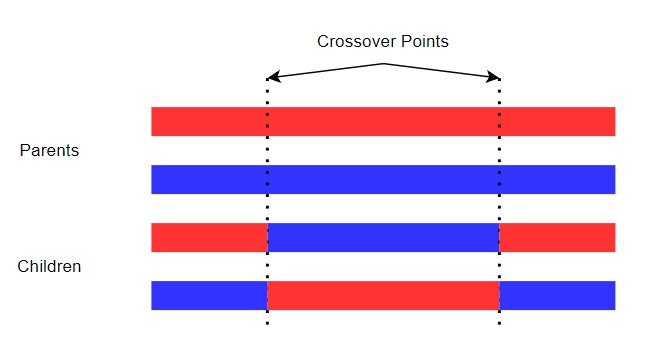
\includegraphics[height=1.5in,width=3in]{2Point}
\caption{Two Point Crossover}
\label{fig:2Point}
\end{figure}
\item[Uniform Crossover] randomly selects which parent's alleles will be copied for each gene. In our experiments, the probability for each parent to be selected is equal. \cite{Belfiore1998}
\end{description}

The advantage granted by two point crossover compared to a single point is that we can search the problem space much more thoroughly and this effect is made stronger with a uniform crossover. However, such a wide search can cause offspring to fail to exploit the genes that granted their parents a high fitness. By choosing three operators that follow the same principle to different effects, we can explore that effect on our stated problem effectively.

\subsubsection{Mutation}
Mutation affects the newly made child individuals and introduces new genetic material to the search space. This allows the population to move to new areas in the search space. A mutation rate parameter is used to determine the probability of the operator taking effect.  We implemented and tested the following operators:
\begin{description}
\item[Swap Mutation] randomly chooses two genes in the individual and swaps their alleles. The chance of mutation occuring is per individual.\cite{Mutation}
\item[Inverse Mutation] randomly selects two positions in the genome and inverts the position of all genes between these positions. The chance of mutation occuring is per individual. \cite{Mutation}
\item[Floating Point Mutation] changes the values of a gene by a set value with an equal chance of the value being added or subtracted. The chance of mutation occuring is per gene. The implementation of this was provided in the coursework.
\end{description}

We explore the effect of altering the chance of mutation occuring and in the case of floating point mutation, we explore the effect of the delta change the mutation causes.

\subsubsection{Replacement}
Replacement is the mechanism by which new child individuals replace existing members in the population.
\begin{description}
\item[Replace Worst] replaces the lowest fitness members of the population with the new child individuals, regardless of the child's fitness. The implementation of this was provided in the coursework.
\item[Replace Worst Parent] replaces a parent individual with the new child individual, only if the child is more fit \cite{replacement}.
\item[Tournament Replacement] selects t individuals from the population and selects the least fit individual to be replaced by the child solution, if the child solution is more fit than the least fit in the tournament.

\end{description}

"Replace Worst" is a very common replacement operator. It allows the population to cull the weakest individuals in the population. When using selection methods such as tournament selection, the weakest individuals are unlikely to ever be selected and so are effectively dead weight. "Replace Worst Parent" puts children up against their presumably high fitness parents. This ensures that progress towards better fitness areas is made by a generation, rather than potentially causing the population to hover over a middling fitness area. However, offspring that are worse than their parents may still contain genetic material that is worthwhile and so this operator may perform more poorly in certain conditions. Lastly, tournament replacement can allow low fitness individuals to survive, allowing their potentially useful genetic information to survive for another generation. It does come with the caveat that we risk eliminating higher fitness individuals if our random selection chooses a group from the higher fitness part of the population.
\subsection{Neural Network Parameters}
Parameters that are changed are the minimum and maximum values of the weights, number of hidden nodes and the activation function.
\subsubsection{Minumum and Maximum Values}
The minimum and maximum values of the weights used in the neural network must be set carefully. Too tight a range of values can cause underfitting and too high a value can cause overfitting. We explore the effect of these values +/-1 from the default value of +/-3 provided in the coursework.

\subsubsection{Hidden Nodes}
Similar to the value of weights, the number of hidden nodes in a neural network can lead to under/overfitting on our training data. We explore this effect by adjusting the number of hidden nodes in the neural network until we see evidence of overfitting.
\subsubsection{Activation Function}
An activation function defines the output of a node in a neural network given an input. We implemented and tested the following activation functions.
\begin{description}
\item[Hyperbolic Tangent] defined as:
\begin{figure}[!htb]
\begin{equation}
f(x) = tanh(x) = \frac{sinh(x)}{cosh(x)}
\end{equation}
\caption{TanH Activation Function}
\label{fig:SoftSign}
\end{figure}

\item[Arc Tangent] defined as:
\begin{figure}[!htb]
\begin{equation}
f(x) = tan{}^{-1}(x)
\end{equation}
\caption{Arc Tangent Activation Function}
\label{fig:SoftSign}
\end{figure}
\item[Soft Sign] defined as:
\begin{figure}[!htb]
\begin{equation}
f(x) = \frac{x}{1+|x|}
\end{equation}
\caption{SoftSign Activation Function}
\label{fig:SoftSign}
\end{figure}
\end{description}

"Hyperbolic Tangent" is provided with the coursework. We chose to implement an arc tangent activation function as the smoother gradient at extreme inputs allows for greater differentiation between inputs. Similarly, "SoftSign" provides this smoothing effect more greatly so we can determine if this effect can have a positive effect in finding an optimal solution.

\section{Experiments \& Analysis}
All results presented are a mean average from ten runs. Unless otherwise specified, all experiments were run with the following setup which was taken from a known good solution discovered during development that had a test data fitness of 0.05.

\begin{center}
\begin{tabular} {|c|c|}
\hline
Operators & Chosen Method \\
\hline
Selection & Tournament Selection \\
Recombination & Two Point Crossover \\
Mutation & Standard \\
Replacement & Worst \\
Activation & TanH \\
\hline
\end{tabular}
\end{center}
\begin{center}
\begin{tabular} {|c|c|}
\hline
Parameters & Values \\
\hline
Hidden Nodes & 10 \\
Min Gene & -3.0 \\
Max Gene & 3.0 \\
Pop Size & 200 \\
Generations & 20000 \\
Tournament Size & 50 \\
Mutation Rate & 0.5 \\
Mutation Change & 1.0 \\

\hline

\end{tabular}
\end{center}

\subsection{Operators}
\subsubsection{Selection}
Presented below are the mean training and test fitness obtained from each of our chosen selection operators. The number in parentheses following "Tournament" indicates the tournament size.
\begin{center}
\begin{tabular} {|c|c|c|}
\hline
Operator & Training Fitness & Test Fitness \\
\hline
Roulette & 0.05109 & 0.0866 \\
Elitist & 0.02981 & 0.08835 \\
Tournament (50) & 0.03071 & 0.08406 \\
Tournament (75) & 0.02449 & 0.08495 \\
Tournament (100) & 0.02526 &  0.06668\\
Tournament (125) & 0.03544 & 0.11092 \\


\hline

\end{tabular}
\end{center}
Applied to our training data set, we have two close best average fitness values provided by our tournament operator with tournament size set to 75 and 100. A tournament size of 100 provides our best test fitness values by some margin. To determine if this is relevant, we first test for normal distribution on our test fitness results obtained with a tournament size of 75 and 100 with a Shapiro-Wilk test (p Values: 75=0.015, 100=0.003) , which indicates a non-normal distribution, and subsequently apply a Mann-Whitney U test to determine if both sets come from the same distribution with a resulting p value of 0.44. This high value indicates that there is no difference in the distribution of these data sets. We therefore conclude that may be no meaningful difference between tournament sizes 75 and 100 and our results are due to variance.

We see a high degredation in test fitness recieved from a tournament size of 125. With such a high tournament size, we are more likely to consistently choose the same parents who are the fittest in the entire population. This would be similar to an "Elitist" operator however we see worse performance that that. This may be due to the fact that unlike "Elitist" there is no protection against the same parent being chosen twice which would result in children which, other than the effects of mutation, would be identical to their parent. This would lead to a dramatic loss in diversity over time, preventing the population from exploring new spaces and and it appears that in practice, the population settles on a good fitness value within a local area resulting an overfitting on the training fitness.

We note that, despite a much worse training fitness, our "Roulette" operator provides very similar results to the other operators when applied to our test data set.
\subsubsection{Recombination}
Presented below are the mean training and test fitness obtained from each of our chosen recombination operators.
\begin{center}
\begin{tabular} {|c|c|c|}
\hline
Operator & Training Fitness & Test Fitness \\
\hline
One Point Crossover & 0.0136 & 0.03565 \\
Two Point Crossover & 0.01342 & 0.02611 \\
Uniform Crossover & 0.02457 & 0.08171 \\

\hline

\end{tabular}
\end{center}

We see best fitness achieved on both sets by "Two Point Crossover". "Uniform Crossover" performs worse on training and considerably worse on test data. With every gene having the chance to be obtained from either parent, each child can be significantly different from their parent. With a high amount of mutation present in our parameters(0.5), this may prevent meaningful exploitation in the area where the parents are present. To test this, we ran our algorithm with a lower mutation rate of 0.2 ten times and obtain a higher mean training and mean test fitness of 0.03 and 0.10 respectively, indicating that this not the case. An alternate explanation would be that the order of the genes and their values is relevant and the high disruption of "Uniform" crossover causes negative effects. Our understanding of the gene sequence of an individual is that for example, the first X weights would be for the first input node times X hidden nodes. The good fitness values displayed by an individual may only be due to these groups of weights working in conjunction which "One Point" and "Two Point" crossover are more likely to retain.

\subsubsection{Mutation}
Presented below are the mean training and test fitness obtained from each of our chosen mutation operators.
\begin{center}
\begin{tabular} {|c|c|c|}
\hline
Operator & Training Fitness & Test Fitness \\
\hline
Swap & 0.05736 & 0.18552 \\
Inverse & 0.09731 & 0.18775 \\
Floating Point & 0.01407 & 0.04243 \\

\hline

\end{tabular}
\end{center}


We find that the floating point mutation operator provided worked best by a large margin. The issue presented by "Swap" and "Inverse" mutation is that they do not introduce new genetic material in floating point representations. Changing the positions of the genetic values allows the search to expand into new environments but these environments are limited to values that already exist in the population preventing true freedom to explore the search space. The issues presented by these operators are less likely to be an issue with a different representation such as in a permutation problem. It was an oversight in design to have included these operators and time spent implementing and testing could have been spent on other useful operators. We suspect that a combination of "Swap"/"Inverse" and floating point mutation could work well but were unable to test this.

Moreover, if our suspicion presented in our commentary on "Uniform Crossover" and the importance of order in the genotype is true then it would indicate that the disruptive effect on order caused by the "Inverse" mutation would be potentially detrimental to fitness.

\subsubsection{Mutation Rate}
As we have discounted "Swap" and "Inverse" operators, we choose to experiment with mutation rate and the delta change caused by the mutation using the provided floating point mutation. Presented below are the mean training and test fitness obtained from a variety of parameters.

\begin{center}
\begin{tabular} {|c|c|c|}
\hline
Mutation Rates& Training Fitness & Test Fitness \\
\hline
0.1 & 0.0358 & 0.11306 \\
0.3 & 0.01104 & 0.03431 \\
0.5 & 0.02479 & 0.0779 \\
0.7 & 0.02554 & 0.07928 \\
0.9 & 0.03035 & 0.08065 \\

\hline

\end{tabular}
\end{center}

\begin{figure}[!htb]
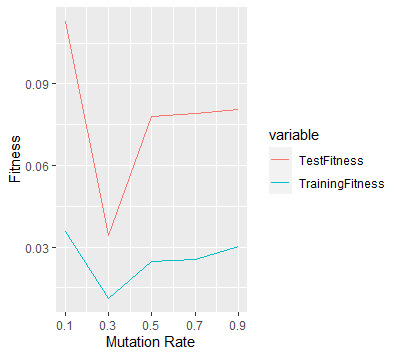
\includegraphics[height=2.5in,width=3in]{MutationRateGraph}
\caption{Mutation Rate Graph}
\label{fig:MutationRateGraph}
\end{figure}
Figure{fig:MutationRateGraph} shows a clear best parameter in a 0.3 mutation rate. We can infer from the worse mutation rate displayed by a 0.5 mutation rate and higher that mutation occuring too often causes children to be too distinct from their parents, preventing meaningful exploitation of the area occupied by the parents. Similarly, we see poor fitness with a 0.1 mutation rate. Such a low rate causes children to be too similar to their parents, causing the population to remain in local optimum areas and missing a potential global optimum.
\subsubsection{Mutation Delta}
\begin{center}
\begin{tabular} {|c|c|c|}
\hline
Mutation Delta& Training Fitness & Test Fitness \\
\hline
0.5 & 0.02555 & 0.07316 \\
1.0 & 0.01602 & 0.06473 \\
1.5 & 0.0231 & 0.0763 \\

\hline

\end{tabular}
\end{center}
We see best results provided by a 1.0 mutation delta. 
Our choice of operator in this experiment demonstrates a failure in design. When a gene is subject to mutation by a set delta, that allele can only shift to a set of possible values which is the original value +/- delta. Through recombination and replacement, that allele can spread to many individuals and the same can be said of all alleles. This means that, with a fixed delta, there exists blind spots in the search space where the population may only search a finite number of spaces, determined by the random values assigned on population initialisation. Potential solutions are discussed in the section \nameref{FutureWork}.

\subsubsection{Replacement}
Presented below are the mean training and test fitness obtained from each of our chosen replacement operators.


\begin{center}
\begin{tabular} {|c|c|c|}
\hline
Operator & Training Fitness & Test Fitness \\
\hline
Replace Worst & 0.01289 & 0.06342 \\
Replace Worst Parent & 0.01486 & 0.04157 \\
Tournament Replacement & 0.035 & 0.0672 \\

\hline

\end{tabular}
\end{center}
Our best fitness on training is obtained by "Replace Worst Parent" and best test is obtained by "Replace Worst".  To determine if this is a meaningful difference, we confirm both results for test fitness come from a normal distribution (Shapiro-Wilks P Values: 0.3 and 0.4) and apply a Welch Two Sample t-Test with a result of 0.19, indicating that there is no difference in their distributions allowing us to assume there is no difference between our experiments.
We see poor performance in training for our "Tournament" replacement operator but similar results to our other operators in test fitness. To determine if our training data result is of significance, we determine that both our "Replace Worst" and "Tournament" training results come from a non-normal distribution (Shapiro-Wilks P Values: 0.005 and 0.002) and apply a Mann-Whitney U Test with a p value result of 0.12, indicating that they come from they come from slightly similar distributions. We therefore conclude that our choice of replacement operator between these is unlikely to make a meaningful difference.


\subsection{Parameters}
\subsubsection{Min/Max Values}
\begin{center}
\begin{tabular} {|c|c|c|}
\hline
Values& Training Fitness & Test Fitness \\
\hline
-2/+2 & 0.01513 & 0.03224 \\
-3/+3 & 0.01503 & 0.0391 \\
-4/+4 & 0.02481 & 0.0934 \\

\hline
\end{tabular}
\end{center}
Our default value of -/+3 performs best in this scenaro. We see -/+4 performs fine on the training set and performs very poorly on the test set. Too extreme a weight assigned to a neuron can cause the output to be nearly fixed regardless of the input in some activation functions such as the tanH function used in this experiment. We suspect such a behaviour begins occuring at this higher value and causes an overfitting to the training set.


\subsubsection{Hidden Nodes}
In this experiment, we alter the number of hidden nodes in the neural network, and therefore the number of genes in an individual, in a step of 5 less than and more than our default value of 10.

\begin{center}
\begin{tabular} {|c|c|c|}
\hline
Hidden Nodes & Training Fitness & Test Fitness \\
\hline
5 & 0.01863 & 0.05944 \\
10 & 0.01441 & 0.05659 \\
15 & 0.01858 & 0.04348 \\

\hline

\end{tabular}
\end{center}

We find that all parameter values provide similar results. Our initial suspicion was that 15 would be too many hidden nodes and would lead to overfitting on our test set. The data suggests this is not the case therefore we ran our experiment again with considerably larger numbers of hidden nodes in order to determine the point at which overfitting will begin to occur.

\begin{center}
\begin{tabular} {|c|c|c|}
\hline
Hidden Nodes & Training Fitness & Test Fitness \\
\hline
20 & 0.01464 & 0.05096 \\
25 & 0.01946 & 0.04501 \\
35 & 0.01534 & 0.03687 \\
50 & 0.01601 & 0.04341 \\
75 & 0.01733 & 0.04129\\
100 & 0.02747 &0.08426 \\
\hline

\end{tabular}
\end{center}

\begin{figure}[!htb]
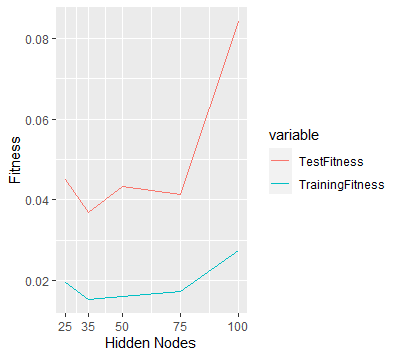
\includegraphics[height=2.5in,width=3in]{NodesGraph}
\caption{Overfitting Effect on High Number of Hidden Nodes}
\label{fig:nodesGraph}
\end{figure}
As demonstrated in Figure \ref{fig:nodesGraph}, a sharp overfitting effect occurs with more than 75 hidden nodes. We see similar performance across all hidden node values tested below this with the expection of 35 which provides better test fitness. We conclude that anything higher than 15 and lower than 100 would provide acceptable performance.
\subsection{Activation Function}

\begin{center}
\begin{tabular} {|c|c|c|}
\hline
Activation Function & Training Fitness & Test Fitness \\
\hline
TanH & 0.01622 & 0.06358 \\
arcTan & 0.01256 & 0.05139 \\
SoftSign & 0.01451 & 0.03532 \\

\hline

\end{tabular}
\end{center}

"SoftSign" provides our best results on test fitness by some margin, despite similar results in training. To determine the significance, we test for normality on "SoftSign" and "arcTan" test fitness values (Shapiro-Wilk p Values: 0.005 and 0.02) finding them to be a non-normal distribution and apply a Mann-Whitney U test with a result of 0.6. This indicates they come from very similar distributions and therefore, our choice of activation function makes little difference. All activation functions implemented share the property of being zero-centred, S-shaped and provide somewhat similar outputs given similar inputs, as seen in Figure \ref{fig:functionGraph}. In hindsight, we should have investigated different activation functions to gain a fuller picture of the effect that an activation function can have.

\begin{figure}[!htb]
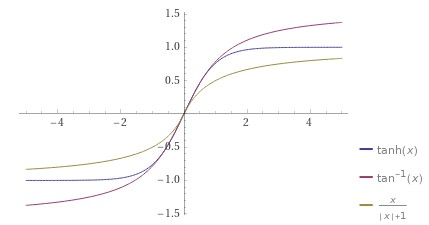
\includegraphics[height=1.5in,width=3in]{activationFunction}
\caption{Activation Function Graph}
\label{fig:functionGraph}
\end{figure}


\section{Conclusions}
Using the best operators and parameters determined via our experiments, we produce the following results:
\begin{center}

\begin{tabular} {|c|c|}
\hline
Data Set & Mean Fitness \\
\hline
Training & 0.01649 \\
Test & 0.04556 \\
\hline

\end{tabular}
\end{center}
\vspace{1em}
\begin{center}
\begin{tabular} {|c|c|}
\hline
Operators & Chosen Method \\
\hline
Selection & Tournament Selection \\
Recombination & Two Point Crossover \\
Mutation & Standard \\
Replacement & Worst Parent \\
\hline
\end{tabular}
\end{center}


\vspace{1em}
\begin{center}

\begin{tabular} {|c|c|}
\hline
Parameters & Values \\
\hline
Hidden Nodes & 15 \\
Min Gene & -3.0 \\
Max Gene & 3.0 \\
Pop Size & 200 \\
Generations & 20000 \\
Tournament Size & 50 \\
Mutation Rate & 0.3 \\
Mutation Change & 1.0 \\
\hline

\end{tabular}

\end{center}
\vspace{1em}


From this set of results, we believe that we have found a near optimal solution that performs extremely well in a variety of situations, achieving a training set fitness of 0.00767 and a test set fitness of 0.00747. Moreover, we achieve a fitness of 0.01175 on the "Go Nuts" set of data demonstrating the flexibility of our best solution, safely landing all ships. When subjected to 10 random runs, all ships safely landed in every run. Due to the high number of genes (138)  in our optimal solution, the generated weights are included with the source code under the folder "bestFound".


While we feel that our best solution is sufficient for the problem, there were mistakes made in the choice of operators, notably our mutation operator and our activation function. More research into how these operators functioned would have better informed our design choices. Possible improvements are discussed in the section Future Work.
We chose to mostly implement well-established operators that work well with more traditional representations such as binary or permutations. Other than the standard floating point mutation operator provided, we did use any operators that could take advantage of the real number representation used.

We see from our experiments on hidden nodes that we do not encounter a strong overfitting effect until over 75 nodes. Such a high number of nodes has a negative effect on runtime so we chose 15 as a compromise.

Overall, our methodical approach to experimentation and testing allowed us to dial in our settings and choice of operators carefully. Our final solution is not perfect, in practice, most ships end with a few units of fuel left over. Other near optimal solutions found could end consistently with no fuel at the cost of a non-centred landing.

\section{Future Work}
\label{FutureWork}
Future attempts at this problem would likely benefit from a mutation operator that utilises a gaussian or cauchy distribution for the mutation delta \cite{Chellapilla1998} to allow greater exploration of the search space. Additionally, experimenting with non-zero centred activation functions such as a rectified linear unit function (ReLU) could provide beneficial effects.

Of note, we also did not experiment with population size which was an oversight. However, we feel that provided the chosen selection operator scales effectively i.e. tournament size scales with population size, this parameter is unlikely to affect fitness found unless set to extremely low values.
Runtime, not counting prohibitively long runtimes, was not considered in this investigation. Our choice to use a steady state algorithm worked well due to the number of iterations used. Were runtime a consideration, an algorithm which replaces more of it's population per generation may be preferable and our findings on optimal settings may not hold water.

\bibliographystyle{ACM-Reference-Format}
\bibliography{bib} 


\end{document}
